\section{Results}

\subsection{Distinctiveness}

\begin{figure*}[t]
\centerline{% 
		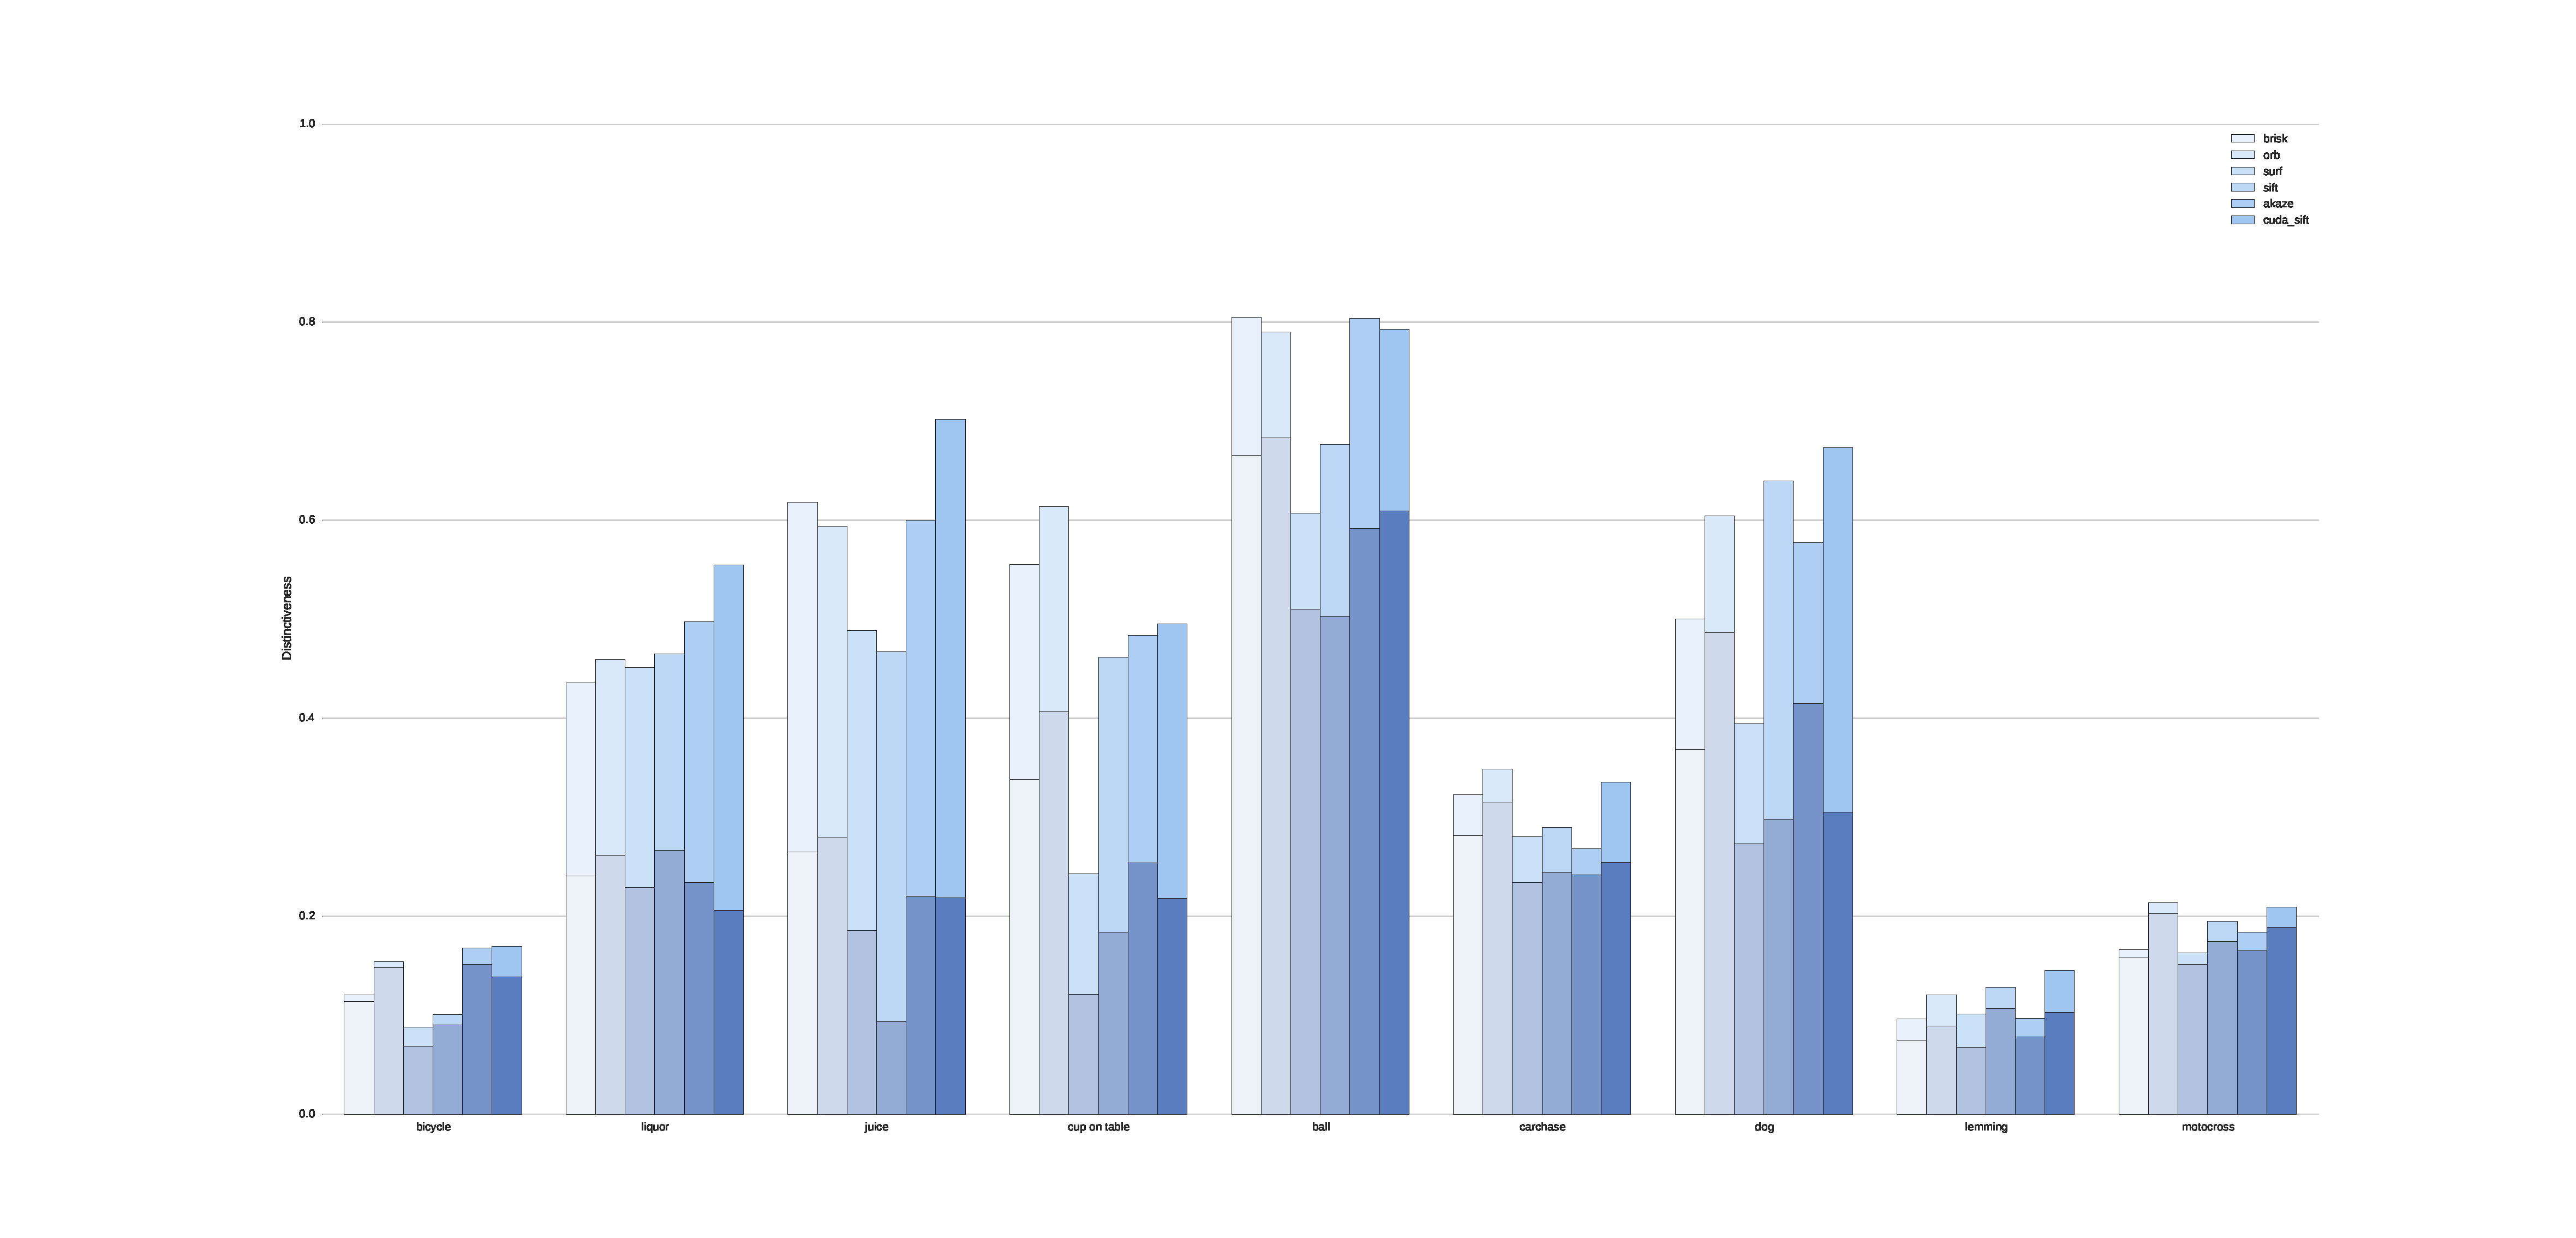
\includegraphics[width=0.98\linewidth]{imgs/distinctivenessTP.pdf}}
    \vspace{-2mm} 
	\caption{Examples take from the dataset showing the ratio of true positives and ambiguous true positives. The lighter color bars show the number of true positives that will actually pass the second best result test.}
	\label{fig:distinctiveness}
\end{figure*}

Fig.~\ref{fig:distinctiveness} shows the amount of true positives and ambiguous true positives for a subset of the videos present in the dataset. the lighter color bars show the number of descriptors that will pass the second best ratio filter. It is interesting to notice that while BRISK and ORB have a higher number of true positives, SIFT and AKAZE present a higher ratio of descriptors that will pass the second best filter. This is an indication that those descriptors are more distinctive. Upon inspection, th number of false positives is comparable as shown in Fig.~\ref{fig:false_positives}.

\begin{figure}[t]
\centerline{% 
		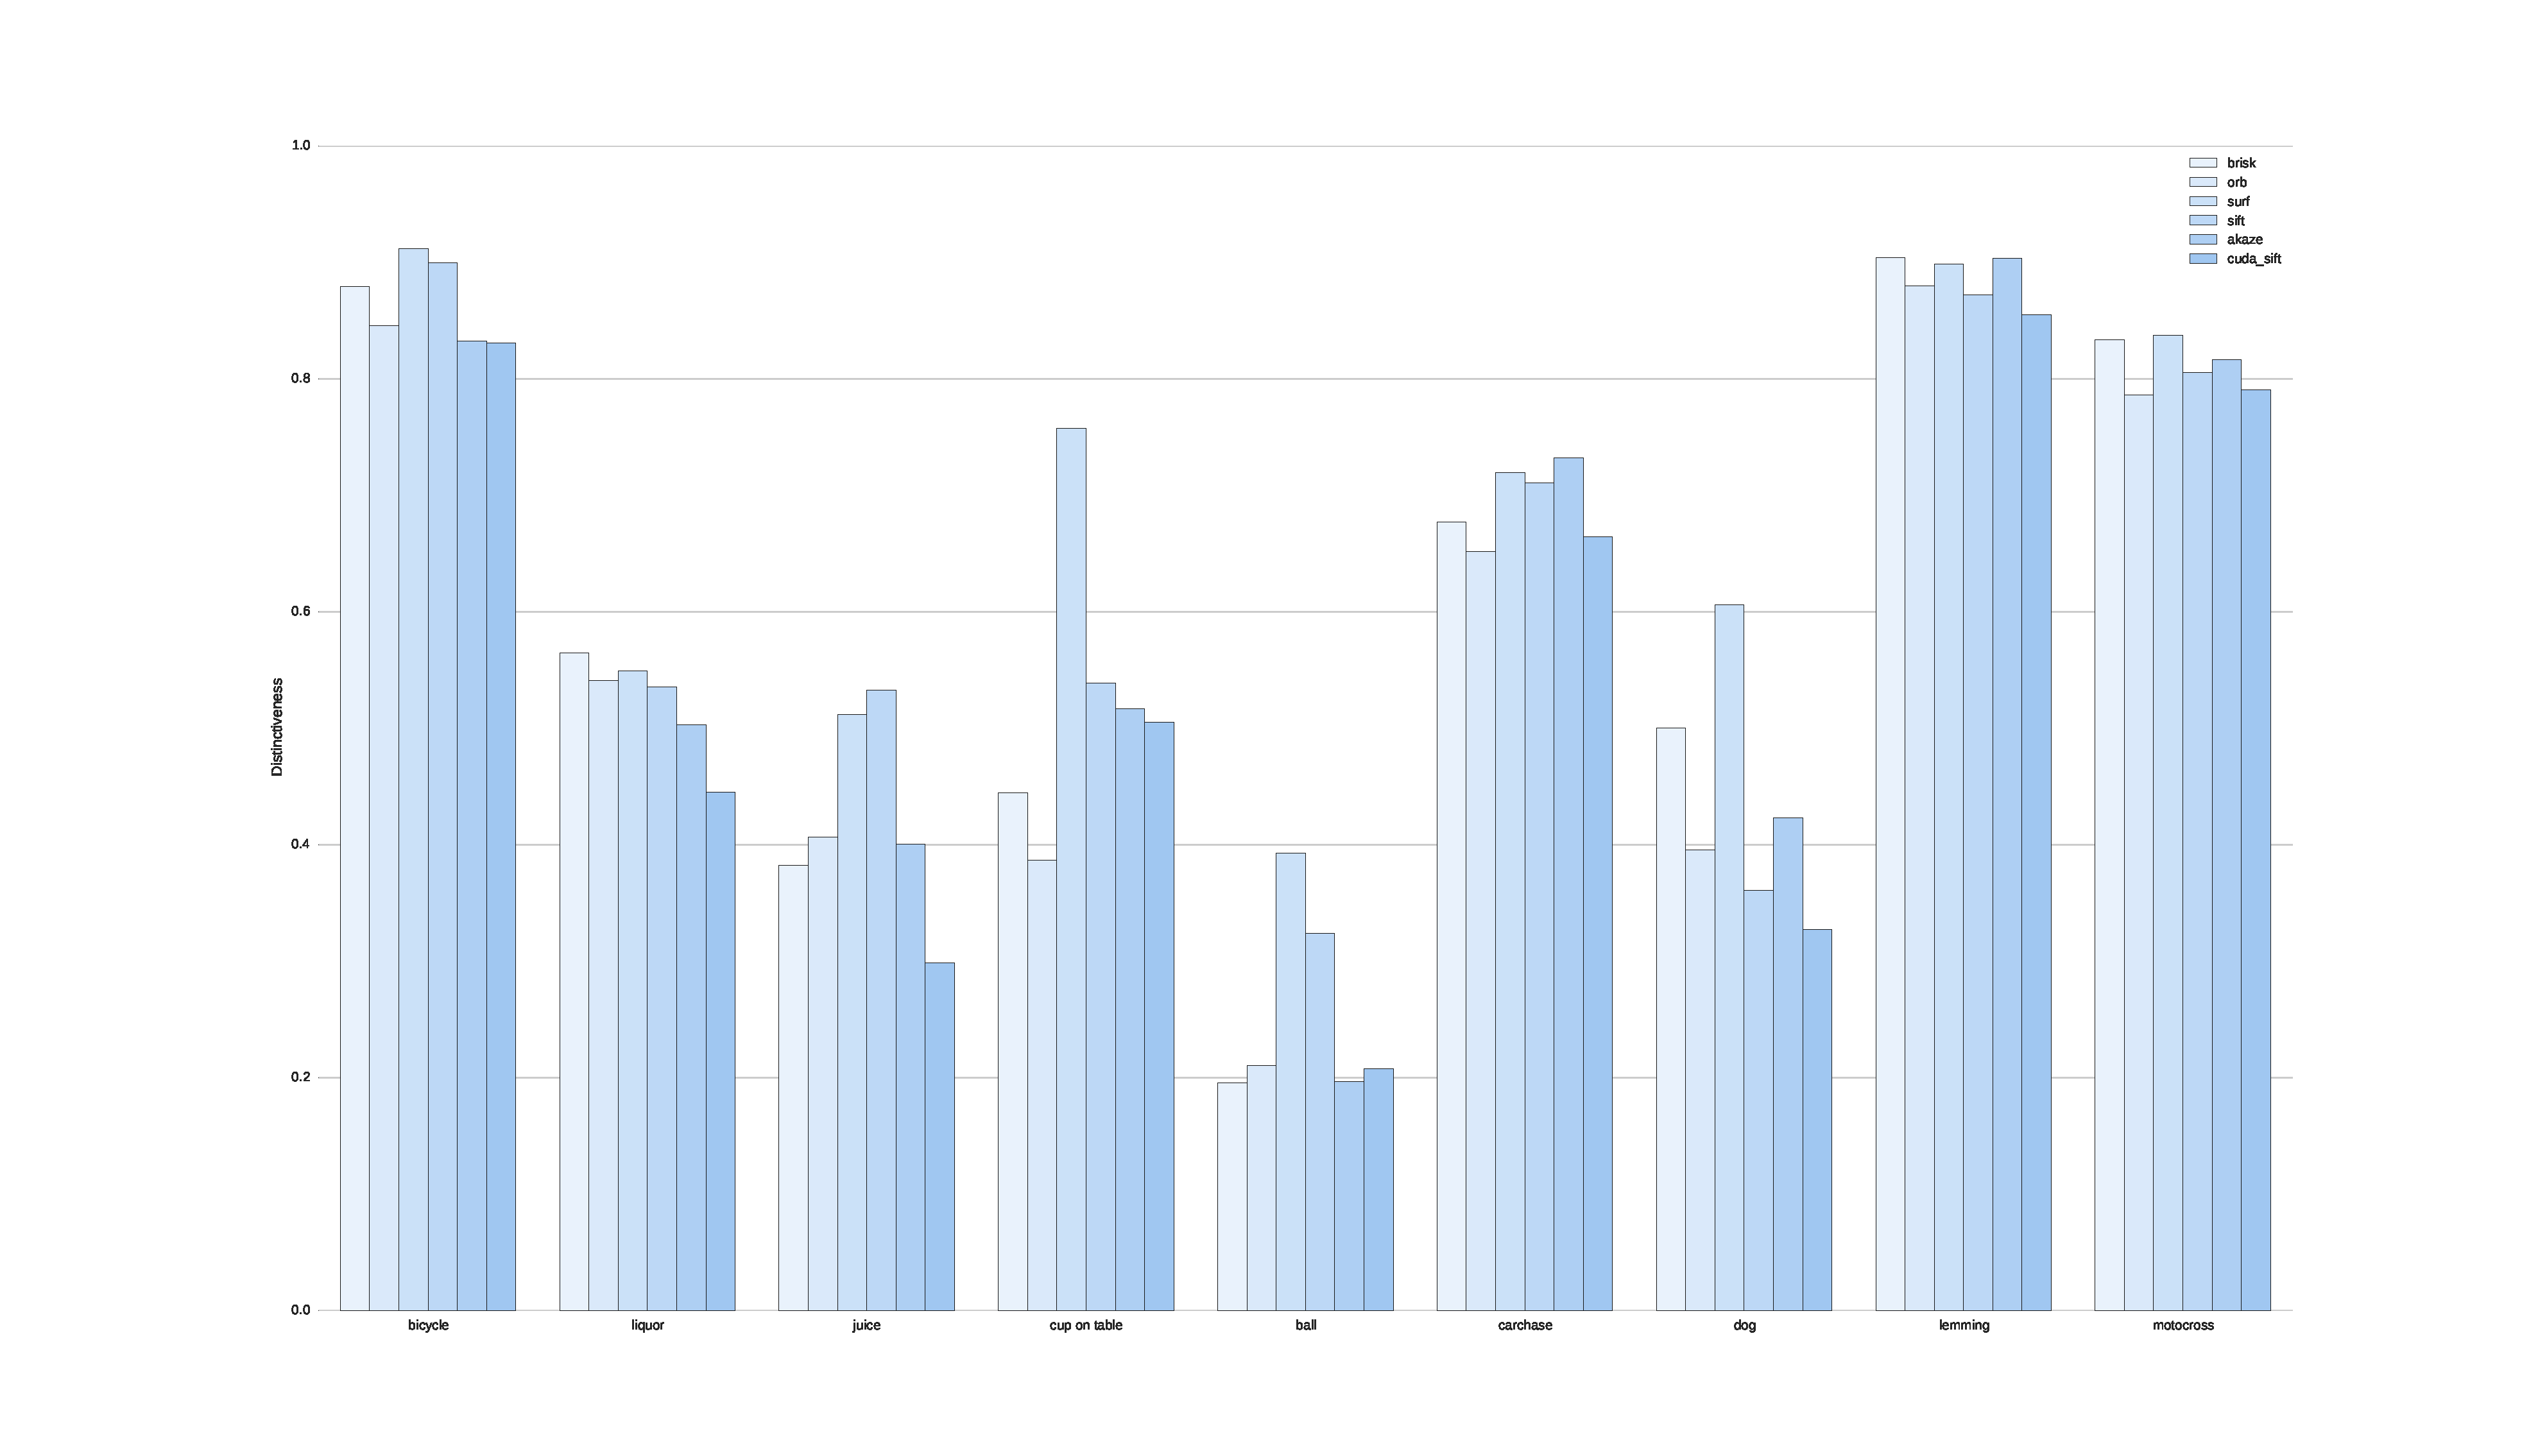
\includegraphics[width=0.98\linewidth]{imgs/false_positives.pdf}}
    \vspace{-2mm} 
	\caption{Examples take from the dataset showing the ratio of true positives and ambiguous true positives. The lighter color bars show the number of true positives that will actually pass the second best result test.}
	\label{fig:false_positives}
\end{figure}


\begin{figure*}[t]
\centerline{% 
		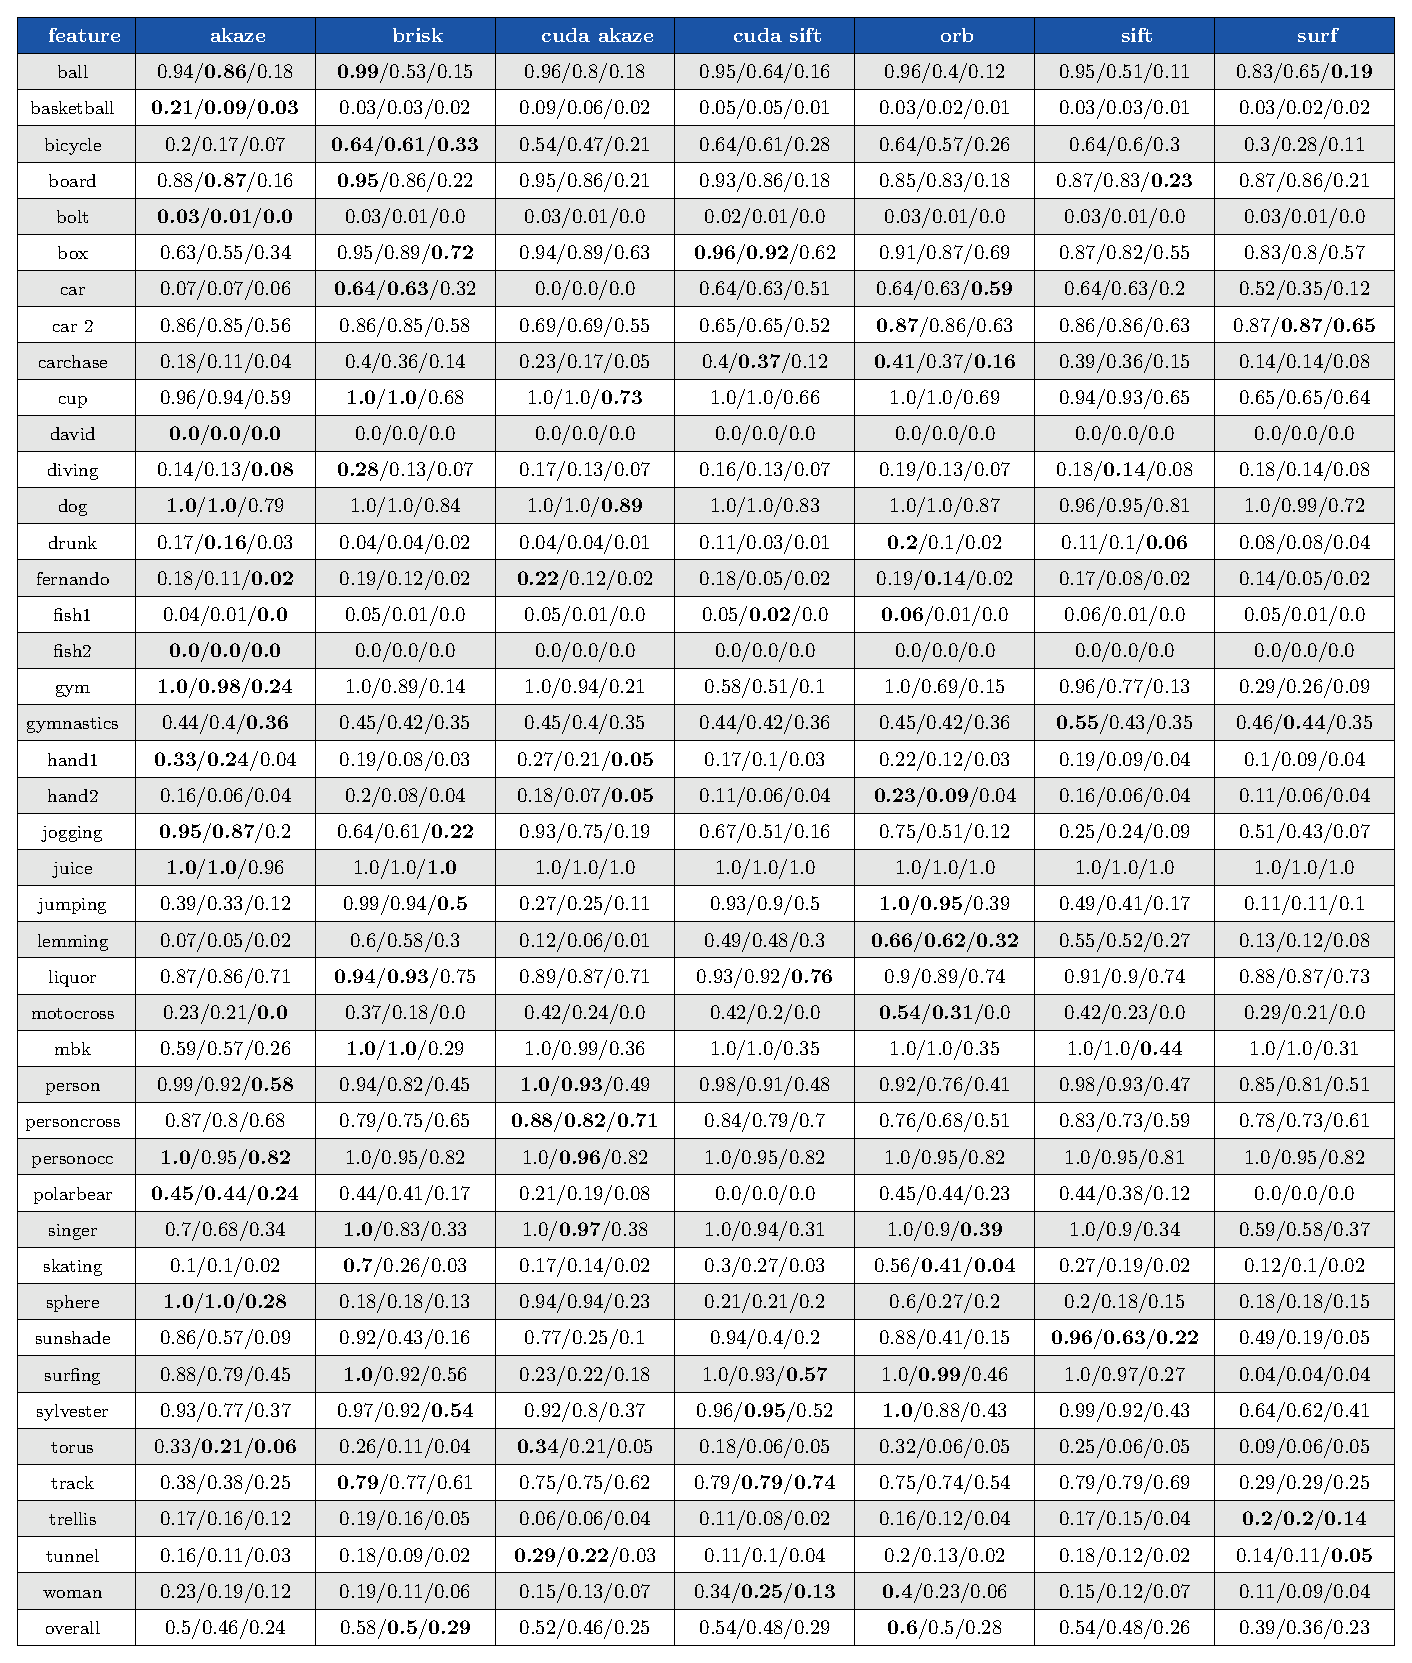
\includegraphics[width=0.98\linewidth]{tables/tracking_precision.pdf}}
    \vspace{-2mm} 
	\caption{Initial tracking results low,medium and high accuracy on all the dataset. Running new experiments on akaze right now with better parameters.}
	\label{fig:false_positives}
\end{figure*}